\documentclass{beamer}

% Set up the template
\setbeamertemplate{frametitle}
  {\begin{centering}\smallskip
   \insertframetitle\par
   \smallskip\end{centering}}
\setbeamertemplate{itemize item}{$\bullet$}
\setbeamertemplate{navigation symbols}{}
\setbeamertemplate{section in toc}[sections numbered]
\setbeamertemplate{footline}[text line]{%
    \hfill\strut{%
        \scriptsize\sf\color{black!60}%
        \quad\insertframenumber
    }%
    \hfill
}

% Set up table of contents
\AtBeginSection[]
{
  \begin{frame}
    \frametitle{Table of Contents}
    \tableofcontents[currentsection]
  \end{frame}
}

% Upper content bar
\useoutertheme[subsection=false]{smoothbars}
%\insertsectionnavigationhorizontal{\paperwidth}{\hskip0pt plus1fill}{\hskip0pt plus1fill}

% Define some colors:
\definecolor{DarkFern}{HTML}{407428}
\definecolor{DarkCharcoal}{HTML}{4D4944}
\colorlet{Fern}{DarkFern!85!white}
\colorlet{Charcoal}{DarkCharcoal!90!white}
\colorlet{LightCharcoal}{Charcoal!50!white}
\colorlet{AlertColor}{orange!80!black}
\colorlet{DarkRed}{red!70!black}
\colorlet{DarkBlue}{blue!70!black}
\colorlet{DarkGreen}{green!70!black}


% Use the colors:
\setbeamercolor{title}{fg=DarkRed}
\setbeamercolor{frametitle}{fg=Fern}
\setbeamercolor{normal text}{fg=Charcoal}
\setbeamercolor{block title}{fg=black,bg=Fern!25!white}
\setbeamercolor{block body}{fg=black,bg=Fern!25!white}
\setbeamercolor{alerted text}{fg=AlertColor}
\setbeamercolor{itemize item}{fg=Charcoal}



\usepackage{hyperref}
\usepackage{graphics}



\title{An Introduction to Subversion}
\author{Flavio Stanchi}
\date{\today}

\begin{document}

\frame{\titlepage}

\section{Introduction}

\subsection{What is Subversion?}

\frame
{
  \frametitle{Features of Subversion}

  \begin{itemize}
  \item It's a version control system
  \item Uses a centralized model:
  	\begin{itemize}
  	\item Server-client approach
  	\item Version merging
	\item With wireless connections everywhere, it's rarely a limitation
  	\end{itemize}
  \item Easy to learn (but slower than Git)
  \item It's free
  \end{itemize}
}

\subsection{How to get Subversion?}

\frame
{
  \frametitle{Getting Subversion}
  
  \begin{itemize}
  \item<1-> Subversion can be found at \url{https://subversion.apache.org}
  \item<2-> Version 1.8 is the last release at this time
  \item<3-> Client for Windows:
  	\begin{itemize}
	\item<3-> TortoiseSVN (free): \url{http://tortoisesvn.net/}
	\end{itemize}
  \item<4-> Clients for Mac:
  	\begin{itemize}
	\item<4-> Xcode (free): \url{https://developer.apple.com/xcode/downloads/}
	\item<4-> Versions (\$): \url{http://versionsapp.com/}
	\end{itemize}
  \item<5-> If you are using Linux \dots 
  		 \uncover<6->{use the terminal!}
  \end{itemize}
}

\frame
{
  \frametitle{Subversion on Cornell servers}
  
  \begin{itemize}
  \item<1-> CISER on RSCH101 and RSCH106 (tested)
  \item<2-> ECCO
  \item<3-> Quick reference guide at \url{http://www2.vrdc.cornell.edu/news/documentation/subversion/}
  \end{itemize}

}

\subsection{Create a repository}

\frame<beamer:0>
{
  \frametitle{Where to create a repository?}
  
  \begin{itemize}
  \item<1-> TeamForge:
  	\begin{itemize}
	\item<1-> Create an account at \url{https://forge.cornell.edu}
	\item<1-> Follow the instructions at \url{http://www.it.cornell.edu/services/subversion/howto/index.cfm}
	\end{itemize}
  \item<2-> GitHub at \url{https://github.com/}
  \item<3-> Use \textit{svnserve} as a lightweight custom server
  \item<4-> Test repository at \url{http://repository.vrdc.cornell.edu/public/test} (When prompted for a login, use `testuser'/`testuser')
  \end{itemize}

}


\section{Concepts}

\subsection{Centralized version control}


\frame
{
  \frametitle{Centralized version control}
  
  \begin{itemize}
  \item<1-> Server-client approach
  	\begin{itemize}
	\item<1-> The repository is located in the server
	\item<2-> No version control over local copies
	\end{itemize}
  \item<3-> Version merging:
  	\begin{itemize}
  	\item<3-> Multiple editors can check out any given file
	\item<3-> Discrepancies are handled upon checkin
	\end{itemize}
  \end{itemize}
  
}

\subsection{Repository structure}

\frame
{
  \frametitle{Generic setup}
  
  \begin{itemize}
  \item<1-> Trunk: contains all the clean code
  \item<1-> Branches: where all initial work occurs
  \item<1-> Tags and releases (optional)
  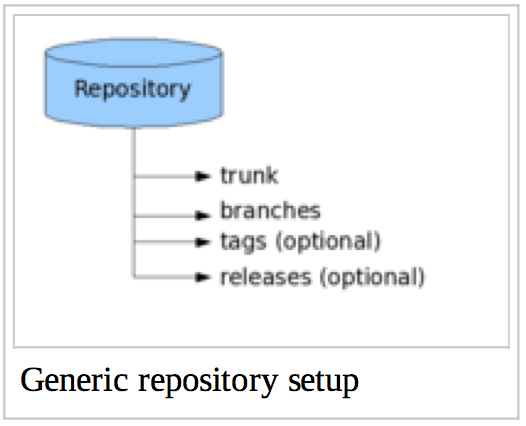
\includegraphics[height=5cm]{repo_structure.png}
  \end{itemize}

}

\subsection{Local copy}

\frame
{
  \frametitle{Local copy}
  
  \begin{itemize}
  \item<1-> The repository may be remote or local \dots 
  		  \uncover<2->{but you don't usually work directly with it}
  \item<3->  Instead, check out a local copy of the repository (or of its subelements)
  \item<4-> Make changes to the local copy
  	\begin{itemize}
	\item<4-> Important: use Subversion commands to do this, so that every change is registered
	\end{itemize}
  \item<5-> Commit the changes back into the repository
  	\begin{itemize}
	\item<5-> Add a commit (log) message
	\item<5-> Every commit is registered with a revision number
	\end{itemize}
  \end{itemize}

}

\frame
{
  \frametitle{Local copy}
  
  \begin{itemize}
  \item<1-> Note: direct changes to the repository are immediately applied \dots
  		  \uncover<2->{while changes to the local copy are applied to the repository upon commit}
  \item<3-> Hence, commit frequently!
  \end{itemize}

}

\subsection{Branches}

\frame
{
	\frametitle{Branches}
	A branch is a line of development that exists independently of another line, yet still shares a common history if you look far enough back in time.\\
	\medskip
	It begins life as a copy of something, and moves on from there, generating its own history.
	
		\begin{figure}[H]
	\centering
	\includegraphics[height=3cm]{branches1.png}
	\end{figure}


}


\frame
{
	\frametitle{Creating a branch}
	Make a copy of (a part of) your project tree in the repository using the \alert{svn copy} command. \\
	\medskip
	The copy may live wherever you wish. Usually, in a folder named \textbf{branches}.\\
	\medskip
	\textbf{Note:} you can do a \alert{remote copy} --- a copy that immediately results in a newly committed repository revision --- no working copy is required! 	Just copy one URL to another.\\
	\medskip
	\alert{Cheap copies:} when you copy a directory, you don't need to worry about duplicating the size, since SVN doesn't actually duplicate any data. Instead, it creates a new directory entry that points to an existing tree.



}

\frame
{
	\begin{figure}[H]
	\centering
	\includegraphics[height=8cm]{branches2.png}
	\end{figure}


}

\section{Workflow}


\subsection{The terminal}

\frame
{
  \frametitle{The terminal}
  
  \begin{itemize}
  \item<1-> On Linux and on OSX, use the terminal
  \item<2-> Advantages:
  	\begin{itemize}
	\item<1-> Flexibility
	\item<2-> It's not so complicated
	\end{itemize}
  \item<3-> Every command must be preceded by \textit{svn}
  
\includegraphics[height=0.8cm]{svn_example.png}
  \end{itemize}
	
}

\subsection{Help}

\frame
{
  \frametitle{Your best friend}
  
  \begin{itemize}
  \item<1-> The most important command is \dots
  		  \uncover<2->{\textit{help}}
  \item<3-> Calling \textit{help} alone will print a summary of the commands and their usage
  \item<4-> Calling \textit{help} followed by the name of a command will print a short description of the command and its options
  \item<5-> Options are often useful (and sometimes necessary), but it's hard to remember them all: use \textit{help}!
  \end{itemize}

}

\subsection{Basic workflow}

\frame
{
  \frametitle{Basic workflow}
  
  \begin{enumerate}
  \item<1-> Update your working copy or check out a new one
  	\begin{itemize}
  	\item<1-> Commands: \textit{co} (\textit{check out}), \textit{update}
  	\end{itemize}
  \item<2-> Make changes
  	\begin{itemize}
	\item<2-> Use your favorite editors
	\item<2-> Commands: \textit{add}, \textit{delete}, \textit{copy}, \textit{move}
	\end{itemize}
  \item<3-> Review the changes
  	\begin{itemize}
	\item<3-> Commands: \textit{status}, \textit{diff}, \textit{log}
	\end{itemize}
  \item<4-> Fix any mistake
  	\begin{itemize}
	\item<4-> Command: \textit{revert}
	\end{itemize}
  \item<5-> Resolve conflicts
  	\begin{itemize}
	\item<4-> Command: \textit{resolve}
	\end{itemize}
  \item<6-> Publish changes
  	\begin{itemize}
	\item<4-> Command: \textit{ci} (commit)
	\end{itemize}
  \end{enumerate}

}

\subsection{Common tasks}

\frame<beamer:0>
{
  \frametitle{Common tasks}
  
  \begin{itemize}
  \item<1-> Accessing a previous version of a file
  	\begin{itemize}
	\item<1-> Commands: \textit{copy}, \textit{export}, with option \textit{-r}
	\end{itemize}
  \item<2-> Identifying changes
  \item<3-> Merging a branch back into the trunk
  \end{itemize}
  
}  


\end{document}